\section{Theorie}

\textbf{\underline{Ziel:}}
Es soll die Funktionsweise eines Lock-In-Verstärkers kennengelernt werden.
\\
\\
Ein Lock-In-Verstärker ist ein Verstärker mit integriertem phasenempfindlichem Detektor und kann für
Messungen verrauschter Signale genutzt werden.
Ein schematischer Aufbau ist in Abbildung \ref{fig:Aufbau1} zu sehen:
\begin{figure}[H]
  \centering
  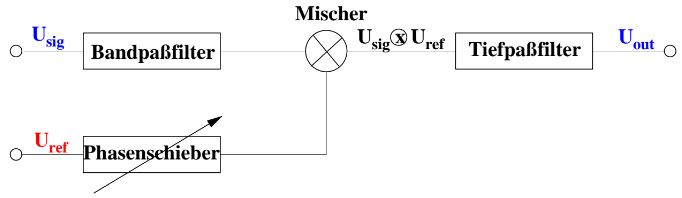
\includegraphics[scale=0.7]{Text/Bilder/LockIn1.jpg}
  \caption{Schematischer Aufbau des Lock-In-Verstärkers \cite[2]{sample}}
  \label{fig:Aufbau1}
\end{figure}
Zunächst wird das Nutzsignal $U_\text{Sig}$ mithilfe eines Bandpassfilters gefiltert.
Dieser befreit $U_\text{Sig}$ von Frequenzen $\omega \gg \omega_\text{0}$ und $\omega \ll \omega_\text{0}$.
Daraufhin wird das Nutzsignal $U_\text{Sig}$ in einem Mischer mit der
Referenzspannung $U_\text{ref}(\omega_\text{0})$ multipliziert.
Die Phasenlage der Referenzspannung kann mit dem Phasenschieber angepasst werden.
Zum Schluss wird das das neu entstandene Signal durch einen Tiefpassfilter geschickt.
Wird eine Referenzspannung durch eine Fourier-Analyse genähert, so muss der Tiefpassfilter so eingestellt sein, dass
die Oberwellen, die sich aus dem Produkt aus Signal- und Modulationsfrequenz ergeben, unterdrückt werden.
Der Tiefpassfilter integriert das Signal über mehrere Perioden und befreit dieses so
von möglichen Störungen, sodass am Ausgang eine
Spannung
\begin{equation}
  U_\text{out} = \frac{2}{\pi}U_\text{0}\cdot \cos{\left(\phi\right)}
  \label{eqn:Uout}
\end{equation}
gemessen werden kann.
Beträgt die Phasenverschiebung 0, so ist die Ausgangsspannung maximal und es gilt:
\begin{equation}
  U_\text{out} = \frac{2}{\pi}U_\text{0}
\end{equation}

%\begin{wrapfigure}{r}{0.45\textwidth}
%  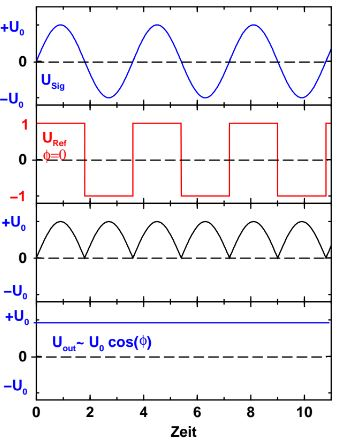
\includegraphics[width=1\linewidth]{Text/Bilder/LockIn2.jpg}
%  \caption{Signalverläufe}
%  \label{fig:Aufbau2}
%\end{wrapfigure}
%In Abbildung \ref{fig:LockIn2} sind die Signalspannung $U_\text{Sig}$, die Refferenzspannung $U_{ref}$ und die Ausgangspannung
%$U_\text{out}$ beispielhaft dargestellt.
